\documentclass[aspectratio=169,11pt]{beamer}
\makeatletter
\NeedsTeXFormat{LaTeX2e}
\ProvidesPackage{beamerthemeDUNEProfessional}[2026/08/19 DUNE professional Beamer theme]

\mode<presentation>

\RequirePackage{iftex}
\RequirePackage{graphicx}
\RequirePackage{xcolor}
\RequirePackage{tikz}
\RequirePackage{adjustbox}
\RequirePackage{array}
\RequirePackage{booktabs}
\RequirePackage{tabularx}
\RequirePackage{ragged2e}

\usetikzlibrary{arrows.meta,calc,fit,positioning,shapes.geometric}

\useinnertheme{default}
\useoutertheme{default}
\usefonttheme{professionalfonts}
\setbeamertemplate{navigation symbols}{}

% Logo path is relative to a deck directory. Override with \DuneSetLogoPath.
\newcommand{\DuneLogoPath}{../../templates/dune-professional/logos}
\newcommand{\DuneSetLogoPath}[1]{\renewcommand{\DuneLogoPath}{#1}}

% Color roles. Keep semantic names in decks; avoid ad hoc local colors.
\definecolor{DuneBg}{HTML}{101820}
\definecolor{DunePanel}{HTML}{1B2733}
\definecolor{DunePanelAlt}{HTML}{263645}
\definecolor{DuneTitleBand}{HTML}{20303E}
\definecolor{DuneLine}{HTML}{536878}
\definecolor{DuneText}{HTML}{F1F5F7}
\definecolor{DuneMuted}{HTML}{BAC6CF}
\definecolor{DuneOrange}{HTML}{F2682B}
\definecolor{DuneCyan}{HTML}{8EDDF2}
\definecolor{DuneMint}{HTML}{9BD7AE}
\definecolor{DuneYellow}{HTML}{E8C85A}
\definecolor{DuneRed}{HTML}{F38B7F}
\definecolor{DuneViolet}{HTML}{B8A7E8}

\setbeamercolor{normal text}{fg=DuneText,bg=DuneBg}
\setbeamercolor{title}{fg=white,bg=DuneBg}
\setbeamercolor{subtitle}{fg=DuneMuted,bg=DuneBg}
\setbeamercolor{author}{fg=DuneCyan,bg=DuneBg}
\setbeamercolor{date}{fg=DuneMuted,bg=DuneBg}
\setbeamercolor{frametitle}{fg=white,bg=DuneBg}
\setbeamercolor{headline}{fg=DuneMuted,bg=DuneBg}
\setbeamercolor{footline}{fg=DuneMuted,bg=DuneBg}
\setbeamercolor{itemize item}{fg=DuneOrange}
\setbeamercolor{itemize subitem}{fg=DuneCyan}
\setbeamercolor{enumerate item}{fg=DuneOrange}
\setbeamercolor{caption name}{fg=DuneMuted}

\setbeamercolor{dune panel}{fg=DuneText,bg=DunePanel}
\setbeamercolor{dune panel alt}{fg=DuneText,bg=DunePanelAlt}
\setbeamercolor{dune accent}{fg=DuneBg,bg=DuneCyan}
\setbeamercolor{dune decision}{fg=DuneBg,bg=DuneYellow}
\setbeamercolor{dune risk}{fg=DuneBg,bg=DuneRed}
\setbeamercolor{dune evidence}{fg=DuneBg,bg=DuneMint}
\setbeamercolor{dune violet}{fg=DuneBg,bg=DuneViolet}

\setbeamerfont{normal text}{size=\small}
\setbeamerfont{title}{series=\bfseries}
\setbeamerfont{subtitle}{size=\large}
\setbeamerfont{author}{size=\normalsize,series=\bfseries}
\setbeamerfont{date}{size=\small}
\setbeamerfont{frametitle}{series=\bfseries}
\setbeamerfont{footline}{size=\scriptsize}

\ifPDFTeX
  \RequirePackage[scaled]{helvet}
  \renewcommand*\familydefault{\sfdefault}
  \RequirePackage[T1]{fontenc}
\else
  \RequirePackage{fontspec}
  \defaultfontfeatures{Ligatures=TeX,Scale=MatchLowercase}
  \IfFontExistsTF{IBM Plex Sans}{
    \setsansfont{IBM Plex Sans}
    \setmainfont{IBM Plex Sans}
  }{
    \IfFontExistsTF{Helvetica Neue}{
      \setsansfont{Helvetica Neue}
      \setmainfont{Helvetica Neue}
    }{
      \IfFontExistsTF{TeX Gyre Heros}{
        \setsansfont{TeX Gyre Heros}
        \setmainfont{TeX Gyre Heros}
      }{
        \IfFontExistsTF{Liberation Sans}{
          \setsansfont{Liberation Sans}
          \setmainfont{Liberation Sans}
        }{
          \setsansfont{DejaVu Sans}
          \setmainfont{DejaVu Sans}
        }
      }
    }
  }
  \IfFontExistsTF{JetBrains Mono}{
    \setmonofont{JetBrains Mono}[Scale=0.88]
  }{
    \IfFontExistsTF{Latin Modern Mono}{
      \setmonofont{Latin Modern Mono}[Scale=0.88]
    }{
      \setmonofont{DejaVu Sans Mono}[Scale=0.88]
    }
  }
  \renewcommand*\familydefault{\sfdefault}
\fi

\setbeamersize{text margin left=0.78cm,text margin right=0.78cm}
\setlength{\leftmargini}{1.15em}
\setlength{\leftmarginii}{1.05em}
\setlength{\parskip}{0.18em}

\setbeamertemplate{itemize item}{%
  \color{DuneOrange}\raisebox{0.15ex}{\scriptsize$\blacktriangleright$}%
}
\setbeamertemplate{itemize subitem}{%
  \color{DuneCyan}\raisebox{0.15ex}{\tiny$\blacktriangleright$}%
}

% Measured boxes: content may shrink down, but never expands outside the safe box.
\newcommand{\DuneFitBox}[3]{%
  \begin{adjustbox}{max width=#1,max totalheight=#2}%
    \begin{minipage}{#1}\raggedright #3\end{minipage}%
  \end{adjustbox}%
}

\newcommand{\DuneTightList}{%
  \setlength{\itemsep}{0.45mm}%
  \setlength{\parskip}{0pt}%
}

\newcommand{\DuneEyebrow}[1]{%
  {\color{DuneCyan}\scriptsize\bfseries #1\par}%
}

\newcommand{\DunePill}[2]{%
  \tikz[baseline=-0.55ex]\node[
    rounded corners=2.5pt,
    draw=#1,
    fill=#1!18!DuneBg,
    inner xsep=4pt,
    inner ysep=1.35pt,
    text=#1,
    font=\tiny\bfseries
  ]{#2};%
}

\newcommand{\DuneCard}[4][dune panel]{%
  \begin{beamercolorbox}[wd=\linewidth,sep=5pt,rounded=true]{#1}
    {\usebeamercolor[fg]{#1}\bfseries #2\par}
    \vspace{0.4mm}
    {\usebeamercolor[fg]{#1}\footnotesize #3\par}
    \if\relax\detokenize{#4}\relax\else
      \vspace{0.5mm}{\usebeamercolor[fg]{#1}\scriptsize #4\par}
    \fi
  \end{beamercolorbox}
}

\newcommand{\DuneFixedCard}[5][dune panel]{%
  \begin{beamercolorbox}[wd=\linewidth,sep=5pt,rounded=true]{#1}
    \begin{minipage}[t][#2][t]{\dimexpr\linewidth-10pt\relax}
      \raggedright
      {\usebeamercolor[fg]{#1}\bfseries #3\par}
      \vspace{0.45mm}
      {\usebeamercolor[fg]{#1}\footnotesize #4\par}
      \if\relax\detokenize{#5}\relax\else
        \vspace{0.55mm}{\usebeamercolor[fg]{#1}\scriptsize #5\par}
      \fi
    \end{minipage}
  \end{beamercolorbox}
}

\newcommand{\DuneFooterLogo}{%
  \IfFileExists{\DuneLogoPath/logosolo.png}{%
    \tikz[baseline=-0.52ex]\node[opacity=0.42,inner sep=0pt]{%
      \includegraphics[height=0.25cm]{\DuneLogoPath/logosolo.png}%
    };%
  }{}%
}

\newcommand{\DuneTalkDate}{%
  \@ifundefined{mydate}{\today}{\mydate}%
}

% Background and fixed frame-title band.
\addtobeamertemplate{background canvas}{%
  \begin{tikzpicture}[remember picture,overlay]
    \fill[DuneBg] (current page.south west) rectangle (current page.north east);
    \draw[DuneLine,line width=0.55pt]
      ($(current page.south west)+(0.78,0.74)$)
      -- ($(current page.south east)+(-0.78,0.74)$);
    \fill[DuneCyan!16]
      ($(current page.south east)+(-3.2,0.83)$) rectangle ++(1.45,0.055);
  \end{tikzpicture}%
}{}

\setbeamertemplate{headline}{}

\setbeamertemplate{frametitle}{%
  \nointerlineskip%
  \begin{tikzpicture}[remember picture,overlay]
    \fill[DuneTitleBand]
      (current page.north west) rectangle ($(current page.north east)+(0,-1.18)$);
    \fill[DuneOrange]
      ($(current page.north west)+(0.78,-0.23)$) rectangle ++(1.38,0.055);
    \node[anchor=west,inner sep=0pt]
      at ($(current page.north west)+(0.78,-0.72)$) {%
        \DuneFitBox{\dimexpr\paperwidth-1.56cm\relax}{6.7mm}{%
          {\color{white}\bfseries\fontsize{17}{20}\selectfont\insertframetitle}%
        }%
      };
    \ifx\insertframesubtitle\@empty\else
      \node[anchor=west,inner sep=0pt]
        at ($(current page.north west)+(0.78,-1.02)$) {%
          \DuneFitBox{\dimexpr\paperwidth-1.56cm\relax}{3.2mm}{%
            {\color{DuneMuted}\scriptsize\insertframesubtitle}%
          }%
        };
    \fi
  \end{tikzpicture}%
  \vspace*{12.5mm}%
}

\setbeamertemplate{footline}{%
  \leavevmode%
  \begin{beamercolorbox}[wd=\paperwidth,ht=6.4mm,dp=1.8mm,leftskip=0.78cm,rightskip=0.78cm]{footline}
    \DuneFooterLogo\hspace{0.45em}{\textcolor{DuneMuted}{\DuneTalkDate}}%
    \hfill%
    {\textcolor{DuneOrange}{\bfseries\insertframenumber}\textcolor{DuneMuted}{/\inserttotalframenumber}}%
  \end{beamercolorbox}%
}

\setbeamertemplate{title page}{%
  \begin{tikzpicture}[remember picture,overlay]
    \fill[DuneBg] (current page.south west) rectangle (current page.north east);
    \fill[DuneTitleBand]
      (current page.north west) rectangle ($(current page.north east)+(0,-3.03)$);
    \fill[DuneOrange]
      ($(current page.north west)+(0.82,-0.58)$) rectangle ++(1.55,0.075);
    \fill[DuneCyan]
      ($(current page.south east)+(-2.8,0.79)$) rectangle ++(1.88,0.065);
    \IfFileExists{\DuneLogoPath/DUNElogo_white.png}{%
      \node[anchor=south east,opacity=0.13,inner sep=0pt]
        at ($(current page.south east)+(-0.55,1.42)$) {%
        \includegraphics[width=0.34\paperwidth]{\DuneLogoPath/DUNElogo_white.png}%
      };
    }{}%
    \IfFileExists{\DuneLogoPath/FNAL-Logo-NAL-Light.png}{%
      \node[anchor=south east,inner sep=0pt]
        at ($(current page.south east)+(-0.92,0.78)$) {%
        \includegraphics[height=0.42cm]{\DuneLogoPath/FNAL-Logo-NAL-Light.png}%
      };
    }{}%
    \node[anchor=north west,inner sep=0pt]
      at ($(current page.north west)+(0.82,-0.88)$) {%
        \DuneFitBox{0.78\paperwidth}{1.48cm}{%
          {\color{white}\bfseries\fontsize{25}{28}\selectfont\inserttitle}%
        }%
      };
    \node[anchor=north west,inner sep=0pt]
      at ($(current page.north west)+(0.82,-3.55)$) {%
        \DuneFitBox{0.56\paperwidth}{1.35cm}{%
          {\color{DuneMuted}\fontsize{13}{17}\selectfont\insertsubtitle}%
        }%
      };
    \node[anchor=north west,text=DuneCyan,font=\bfseries,inner sep=0pt]
      at ($(current page.north west)+(0.82,-6.3)$) {\insertauthor};
    \node[anchor=north west,text=DuneMuted,font=\small,inner sep=0pt]
      at ($(current page.north west)+(0.82,-6.82)$) {\insertdate};
  \end{tikzpicture}%
  \vfill%
}

\tikzset{
  dune repo/.style={
    draw=DuneCyan,
    fill=DuneCyan!12!DunePanel,
    text=DuneText,
    rounded corners=3pt,
    align=center,
    text width=2.35cm,
    minimum height=0.86cm,
    inner sep=4pt,
    font=\scriptsize\bfseries
  },
  dune repo muted/.style={
    draw=DuneLine,
    fill=DunePanelAlt,
    text=DuneText,
    rounded corners=3pt,
    align=center,
    text width=2.35cm,
    minimum height=0.86cm,
    inner sep=4pt,
    font=\scriptsize\bfseries
  },
  dune artifact/.style={
    draw=DuneMint,
    fill=DuneMint!13!DunePanel,
    text=DuneText,
    rounded corners=3pt,
    align=center,
    text width=2.35cm,
    minimum height=0.86cm,
    inner sep=4pt,
    font=\scriptsize\bfseries
  },
  dune decision node/.style={
    draw=DuneYellow,
    fill=DuneYellow!14!DunePanel,
    text=DuneText,
    rounded corners=3pt,
    align=center,
    text width=2.35cm,
    minimum height=0.86cm,
    inner sep=4pt,
    font=\scriptsize\bfseries
  },
  dune flow/.style={-Latex,draw=DuneCyan,line width=0.85pt},
  dune relation/.style={draw=DuneMuted,line width=0.65pt},
  dune evidence flow/.style={-Latex,draw=DuneViolet,dashed,line width=0.85pt},
  dune label/.style={
    fill=DuneBg,
    text=DuneMuted,
    inner sep=1.5pt,
    font=\tiny,
    align=center
  }
}

\mode<all>

\expandafter\patchcmd\csname beamer@@tmpl@title page\endcsname
  {(-2.8,0.79)}{(-2.8,0.50)}{}
  {\PackageError{pds-story}{Could not lower the title rule}{Check the shared title template.}}
\expandafter\patchcmd\csname beamer@@tmpl@title page\endcsname
  {1.48cm}{2.05cm}{}
  {\PackageError{pds-story}{Could not expand the title box}{Check the shared title template.}}
\makeatother
\DuneUseReadableOrange
\renewcommand{\DuneDiagramCaption}[1]{%
  {\color{DuneTextMuted}\footnotesize #1\par}%
}
\title{PDS data acquisition and\\local trigger conditions for VD LE}
\subtitle{single photoelectron activity expectations\\and mitigation strategies}
\author{Manuel Arroyave}
\date{17 September 2026}
\newcommand{\mydate}{17 September 2026}
\hypersetup{colorlinks=true,urlcolor=DuneSky,linkcolor=DuneSky}

% Drawings are explanatory, not simulated or measured waveforms.
\tikzset{
  storybox/.style={rounded corners=3pt,inner sep=10pt,align=center,
    text=DuneOnAccent,font=\normalsize},
  storyarrow/.style={-Latex,line width=1.4pt,draw=DuneSky}
}
% Simplified from the measured Waffles NP02 cathode-C SPE template:
% a narrow maximum followed by a long, curved recovery.
\newcommand{\SiPMPulse}[3]{%
  \begin{scope}[shift={(#1,#2)},yscale=#3]
    \draw[DuneSky,line width=1.35pt]
      (-0.25,0) -- (-0.08,0.01)
      .. controls (-0.035,0.08) and (-0.018,0.82) .. (0,0.98)
      .. controls (0.018,1.04) and (0.045,1.03) .. (0.065,0.96)
      .. controls (0.10,0.78) and (0.16,0.61) .. (0.25,0.47)
      .. controls (0.39,0.29) and (0.56,0.17) .. (0.78,0.09)
      .. controls (1.02,0.035) and (1.30,0.012) .. (1.58,0.004);
  \end{scope}%
}

\begin{document}
\begin{frame}[plain]\titlepage\end{frame}

% 2 -- Starting point.
\begin{frame}{Current DAPHNE gateware: 1024 samples per frame}
  \relax
  {\large DAPHNE samples each channel continuously at the AFE level:\\
  62.5 MSPS $\times$ 14 bits = 875 Mbit/s/channel.\par}
  \bigskip
  \centering
  \begin{tikzpicture}[x=1cm,y=1cm]
    % A selected interval in a continuous input, not one frame per photon.
    \fill[DuneSky!12!DuneBackground] (0.9,0.9) rectangle (3.95,2.35);
    \draw[DuneBorder] (0.05,1.15) -- (4.7,1.15);
    % Small baseline variation plus SiPM-like fast-rise, slow-decay pulses.
    \begin{scope}
      \clip (0.05,1.02) rectangle (4.70,2.35);
      \draw[DuneSky!65,line width=0.75pt]
        (0.05,1.15) -- (0.18,1.17) -- (0.30,1.14) -- (0.43,1.16)
        -- (0.58,1.14) -- (0.73,1.16) -- (0.88,1.15)
        -- (4.70,1.15);
      \SiPMPulse{0.50}{1.15}{0.48}
      \SiPMPulse{1.34}{1.15}{0.98}
      \SiPMPulse{2.42}{1.15}{0.70}
      \SiPMPulse{3.20}{1.15}{0.50}
      \SiPMPulse{4.25}{1.15}{0.66}
    \end{scope}
    \node[text=DuneText,anchor=south west,font=\small] at (0.05,2.7) {Local frame accepted};
    \draw[-Latex,DunePaper,line width=1.1pt] (1.16,2.65) -- (1.16,1.65);
    \draw[DuneSky,|-|] (0.9,0.68) -- (3.95,0.68);
    \node[text=DuneTextMuted,font=\small,anchor=north] at (2.425,0.53)
      {1024 S / 16.384 \(\mu\)s};
    \draw[storyarrow] (4.78,1.65) -- (5.30,1.65);

    % Both fields belong to one frame; this is not a wire-order diagram.
    \draw[DuneBorder,rounded corners=3pt,line width=1pt]
      (5.45,0.42) rectangle (10.03,2.98);
    \node[text=DuneText,font=\bfseries] at (7.74,2.63) {One frame};
    \fill[DuneCoral,rounded corners=2pt] (5.67,1.48) rectangle (9.81,2.15);
    \node[text=DuneOnAccent] at (7.74,1.815) {Up to 5 peak descriptors};
    \fill[DuneSky,rounded corners=2pt] (5.67,0.66) rectangle (9.81,1.33);
    \node[text=DuneOnAccent] at (7.74,0.995) {1024 waveform samples};
    \draw[storyarrow] (10.07,1.65) -- (11.08,1.65);
    \node[text=DuneTextMuted,font=\small,anchor=north] at (10.57,1.36) {Together};
    \node[storybox,fill=DunePaper,text width=1.65cm,inner sep=8pt]
      at (12.33,1.65) {\textbf{DAQ}\\[3pt]Data\\acquisition};
  \end{tikzpicture}\par\bigskip
  \DuneDiagramCaption{Frame = saved samples + peak summaries. A descriptor reports pulse timing and size.}
  \medskip
  {\small\color{DuneTextMuted}
    Baseline: \texttt{daphne-os} + \texttt{daphne-firmware}; self-trigger \texttt{3f17f1b}.}
\end{frame}

% 3 -- Descriptor capacity is distinct from waveform retention.
\begin{frame}{Five summaries may not describe every peak}
  \centering
  \begin{tikzpicture}[x=1cm,y=1cm]
    \node[text=DuneSky,font=\bfseries,anchor=west] at (0,4.15) {Waveform sent};
    \node[text=DuneTextMuted,font=\small,anchor=east] at (13.6,4.15)
      {One 1024-sample frame};
    \draw[DuneBorder,rounded corners=2pt] (0,2.02) rectangle (13.6,3.87);
    \draw[DuneBorder] (0.2,2.24) -- (13.4,2.24);
    % One frame with seven resolved, SiPM-like pulses.
    \begin{scope}
      \clip (0.2,2.05) rectangle (13.4,3.85);
      \draw[DuneSky!65,line width=0.75pt]
        (0.2,2.24) -- (0.45,2.26) -- (0.68,2.23) -- (0.92,2.25)
        -- (2.58,2.24) -- (4.48,2.24) -- (6.38,2.24)
        -- (8.28,2.24) -- (10.18,2.24) -- (12.08,2.24) -- (13.4,2.24);
      \foreach \x/\a in {1.0/0.88,2.9/0.66,4.8/1.05,6.7/0.75,8.6/0.94,10.5/0.70,12.4/0.86} {
        \SiPMPulse{\x}{2.24}{\a}
      }
    \end{scope}
    \foreach \x/\n in {1.0/1,2.9/2,4.8/3,6.7/4,8.6/5,10.5/6,12.4/7} {
      \node[text=DuneSky,font=\small] at (\x,3.57) {\n};
    }
    \node[text=DuneCoral,font=\bfseries,anchor=west] at (0,1.46) {Peak descriptors sent};
    \foreach \x/\n in {1.0/1,2.9/2,4.8/3,6.7/4,8.6/5} {
      \node[fill=DuneCoral,text=DuneOnAccent,rounded corners=2pt,
        minimum width=1.48cm,minimum height=0.67cm] at (\x,0.67) {Peak \n};
    }
    \node[text=DuneText,align=center,text width=3.1cm] at (11.45,0.67)
      {Peaks 6 and 7:\\no descriptor};
  \end{tikzpicture}\par\medskip
  {\large All seven peaks remain in the waveform.\\Only five have a summary.\par}
  \medskip
  \DuneDiagramCaption{Illustrative resolved peaks; numbers identify peaks, not photoelectron counts.}
\end{frame}

% 4 -- Builder busy and output-queue admission are distinct rejection causes.
\begin{frame}{Dead time can continue after the frame is complete}
  \centering
  \begin{tikzpicture}[x=1cm,y=1cm]
    \fill[DuneSky] (0.55,0.85) rectangle (5.05,1.92);
    \node[text=DuneOnAccent,align=center] at (2.80,1.385)
      {Assembling the\\1024-sample frame};
    \fill[DuneCoral] (5.05,0.85) rectangle (10.80,1.92);
    \node[text=DuneOnAccent,align=center] at (7.925,1.385)
      {Next frame still blocked\\by queued output data};
    \fill[DuneSurfaceRaised] (10.80,0.85) rectangle (13.30,1.92);
    \node[text=DuneText,align=center] at (12.05,1.385) {Can accept\\a new frame};

    \draw[-Latex,DunePaper,line width=1.3pt] (0.55,2.94) -- (0.55,2.02);
    \node[text=DunePaper,anchor=south west,font=\small] at (0.20,3.00) {Accepted};
    \draw[-Latex,DuneTextMuted,line width=1.3pt] (3.05,2.94) -- (3.05,2.02);
    \node[text=DuneTextMuted,anchor=south,font=\small] at (3.05,3.00) {Rejected};
    \foreach \x in {6.30,8.25,9.80} {
      \draw[-Latex,DuneCoral,line width=1.3pt] (\x,2.94) -- (\x,2.02);
    }
    \node[text=DuneCoral,anchor=south,font=\small] at (8.05,3.00)
      {Later triggers also rejected};
    \draw[DunePaper,densely dashed] (5.05,0.61) -- (5.05,2.25);
    \node[text=DunePaper,align=center,anchor=north,font=\small] at (5.05,0.48)
      {Frame\\complete};
    \draw[DuneTextMuted,densely dashed] (10.80,0.61) -- (10.80,2.25);
    \node[text=DuneTextMuted,align=center,anchor=north,font=\small] at (10.80,0.48)
      {Queue below\\admission limit};
    \draw[storyarrow] (0.20,-0.60) -- (13.30,-0.60);
    \node[text=DuneTextMuted,anchor=north east,font=\small] at (13.30,-0.70) {Time};
  \end{tikzpicture}\par\medskip
  {\large A full output FIFO can block the next frame long after assembly ends.\par}
  \medskip
  \DuneDiagramCaption{Illustrative congested case, not to scale. The extra wait depends on how quickly shared readout drains the queue.}
\end{frame}

% 5 -- Capture dead time excludes signal already saved in a waveform.
\begin{frame}{Count the time when signal cannot be saved}
  \centering
  \begin{tikzpicture}[x=1cm,y=1cm]
    \fill[DuneSky,rounded corners=2pt] (0,1.1) rectangle (5.8,2.1);
    \fill[DuneCoral] (5.8,1.1) rectangle (7.8,2.1);
    \fill[DuneSky,rounded corners=2pt] (7.8,1.1) rectangle (13,2.1);
    \node[text=DuneOnAccent] at (2.9,1.6) {Saved in the first frame};
    \node[text=DuneOnAccent,align=center] at (6.8,1.6) {Uncaptured\\gap};
    \node[text=DuneOnAccent] at (10.4,1.6) {Saved in the next frame};
    \foreach \x in {1.2,9.0} {
      \draw[-Latex,DunePaper,line width=1.1pt] (\x,3.1) -- (\x,2.18);
    }
    \node[text=DuneText,font=\small,anchor=south] at (1.2,3.15) {Frame accepted};
    \node[text=DuneText,font=\small,anchor=south] at (9.0,3.15) {Next frame accepted};
    \draw[DunePaper,densely dashed] (9.0,1.12) -- (9.0,2.1);
    \draw[DuneSky,|-|] (7.8,0.84) -- (9.0,0.84);
    \node[text=DuneTextMuted,font=\small,anchor=east] at (7.55,0.84)
      {Recovered by pretrigger};
    \draw[DuneTextMuted,|-|,line width=1pt] (1.2,0.05) -- (9.0,0.05);
    \node[text=DuneTextMuted,font=\small,anchor=north] at (5.1,-0.08)
      {New-frame requests blocked};
  \end{tikzpicture}\par\medskip
  {\large Dead time = blocked, uncaptured time / observation time.\par}
  \medskip
  \DuneDiagramCaption{A rejected request is not necessarily lost light: its signal may already be in a saved frame.}
\end{frame}

% 6 -- Motivation, method and one result all support the missing-rate question.
\begin{frame}{We needed an activity estimate for each VD channel}
  \relax
  {\large Without an agreed vertical-drift (VD) forecast,\\
    we simulated atmospheric argon and gamma backgrounds.\par}
  \bigskip
  \begin{columns}[c,onlytextwidth]
    \begin{column}{0.55\textwidth}
      \DuneNumberBlock{sky}{87 kHz}{per channel at 0.7 PE}
        {VD cathode estimate, before firmware losses.}
    \end{column}
    \begin{column}{0.40\textwidth}
      {\large A candidate is a pulse\\above the chosen threshold.\par}
    \end{column}
  \end{columns}
  \bigskip
  {\small\color{DuneTextMuted}Study reference: intrinsic backgrounds; eight LArSoft windows; threshold $>0.7$ photoelectrons.\\
    87 kHz/channel is the rounded cathode mean, not a uniform rate across VD. Gammas were studied separately.}
\end{frame}

% 7 -- A fixed output budget bounds every local improvement.
\begin{frame}{One link is still the bottleneck}
  \relax
  {\large Current agreement: one link per board.\par}
  \bigskip
  \centering
  \begin{tikzpicture}[x=0.54cm,y=1cm]
    \fill[DunePaper] (0,1.8) rectangle (15.974,2.4);
    \fill[DuneSky] (0,0.7) rectangle (11.435,1.3);
    \node[text=DuneOnAccent,anchor=west] at (0.2,2.1) {1024 samples};
    \node[text=DuneOnAccent,anchor=west] at (0.2,1.0) {512 samples};
    \node[text=DunePaper,anchor=west] at (16.7,2.1) {16.0 Gbit/s};
    \node[text=DuneSky,anchor=west] at (12.2,1.0) {11.4 Gbit/s};
    \draw[DuneCoral,densely dashed,line width=1.5pt] (7.931624,1.65) -- (7.931624,2.65);
    \draw[DuneCoral,densely dashed,line width=1.5pt] (7.868852,0.55) -- (7.868852,1.55);
    \node[text=DuneCoral,anchor=south,align=center] at (9.7,2.95)
      {Frame-data limits into Hermes:\\7.932 Gbit/s (1024) / 7.869 Gbit/s (512)};
  \end{tikzpicture}\par\medskip
  \DuneDiagramCaption{32 cathode channels at about 87 kHz/channel, threshold $>0.7$ PE. Demand after the local busy gate\\
    (33.62 / 46.53 kframes/s/channel), before shared FIFO losses. Red: frame-data limits with output ready.}
\end{frame}

% 8 -- Separate rate sensitivity from the measured VD trace replay.
\begin{frame}{Limited output capacity drives dead time up}
  \centering
  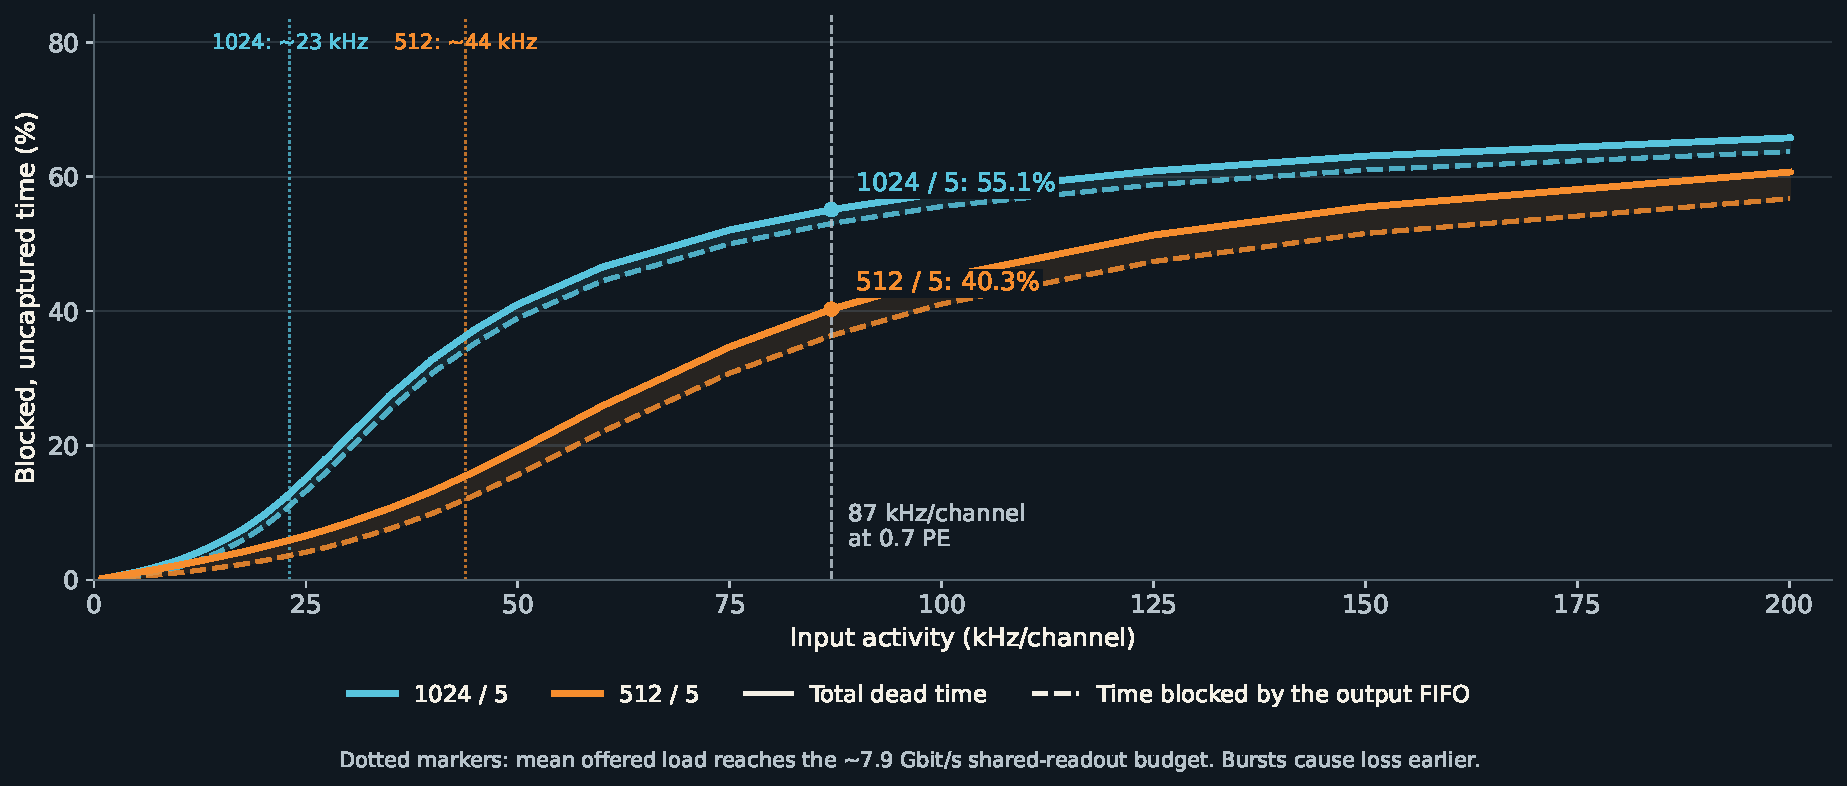
\includegraphics[height=0.64\textheight,width=0.99\linewidth,keepaspectratio]{figures/frequency_deadtime.pdf}\par
  \vspace{0.05cm}
  {\scriptsize\color{DuneTextMuted}
    32 channels/board; one link; matched Poisson inputs. Reference: 87 kHz/channel at 0.7 PE.\\
    Finite shared readout into Hermes; dashed curves count FIFO-blocked, uncaptured time. Additional Hermes/UDP stalls are not simulated.}
\end{frame}

% 9 -- One infrastructure tradeoff; no claim that two links are sufficient.
\begin{frame}{More links buy capacity, with an infrastructure cost}
  \begin{columns}[T,onlytextwidth]
    \begin{column}{0.30\textwidth}
      \DuneNumberBlock{paper}{1 link}{7.869 Gbit/s}{Current agreement}
    \end{column}
    \begin{column}{0.30\textwidth}
      \DuneNumberBlock{sky}{2 links}{15.738 Gbit/s}{Option to study}
    \end{column}
    \begin{column}{0.30\textwidth}
      \DuneNumberBlock{sky}{4 links}{31.475 Gbit/s}{Option to study}
    \end{column}
  \end{columns}
  \bigskip
  {\large Waveforms and peak descriptors share this bandwidth.\par}
  \medskip
  {\large The price: more DAQ servers and power capacity\\in the Central Utility Cavern (CUC).\par}
  \medskip
  {\small\color{DuneTextMuted}512-sample sender budget into Hermes, including scan/pause cycles.\\Balanced load, output ready; network overhead excluded.}
\end{frame}

% 10 -- The implemented gapless path supports the four-link frame-data budget.
\begin{frame}{Four links meet the 256 / 5 frame-data budget}
  \centering
  \begin{tikzpicture}[x=1cm,y=1cm]
    % Frame contents only: no implied sequence, capture duty cycle or wire timing.
    \node[text=DuneText,font=\large\bfseries] at (6.6,3.85)
      {One accepted frame};
    \draw[DuneBorder,rounded corners=3pt,line width=1pt]
      (1.2,0.25) rectangle (12,3.38);
    \node[text=DuneCoral,font=\bfseries] at (6.6,2.96)
      {Up to 5 peak descriptors};
    \foreach \x/\n in {2.4/1,4.5/2,6.6/3,8.7/4,10.8/5} {
      \node[fill=DuneCoral,text=DuneOnAccent,rounded corners=2pt,
        minimum width=1.75cm,minimum height=0.68cm] at (\x,2.28)
        {Slot \n};
    }
    \fill[DuneSky,rounded corners=2pt] (1.52,0.58) rectangle (11.68,1.66);
    \node[text=DuneOnAccent,align=center] at (6.6,1.12)
      {\textbf{256 waveform samples}\\4.096 \(\mu\)s};
  \end{tikzpicture}\par\bigskip
  {\large Each link needs 7.875 Gbit/s. Gapless readout allows 8 Gbit/s.\par}
  \medskip
  \DuneDiagramCaption{Frame data into Hermes: 32 channels across four balanced links.\\Full-load budget; sustained Ethernet/DAQ delivery still needs validation.}
  \medskip
  {\small\color{DuneCoral}256 / 5 loss under the VD activity trace has not been measured.}
\end{frame}

% 11 -- Adapted from the grouped32 continuation illustration.
\begin{frame}{The next frame keeps the pulse's tail}
  \centering
  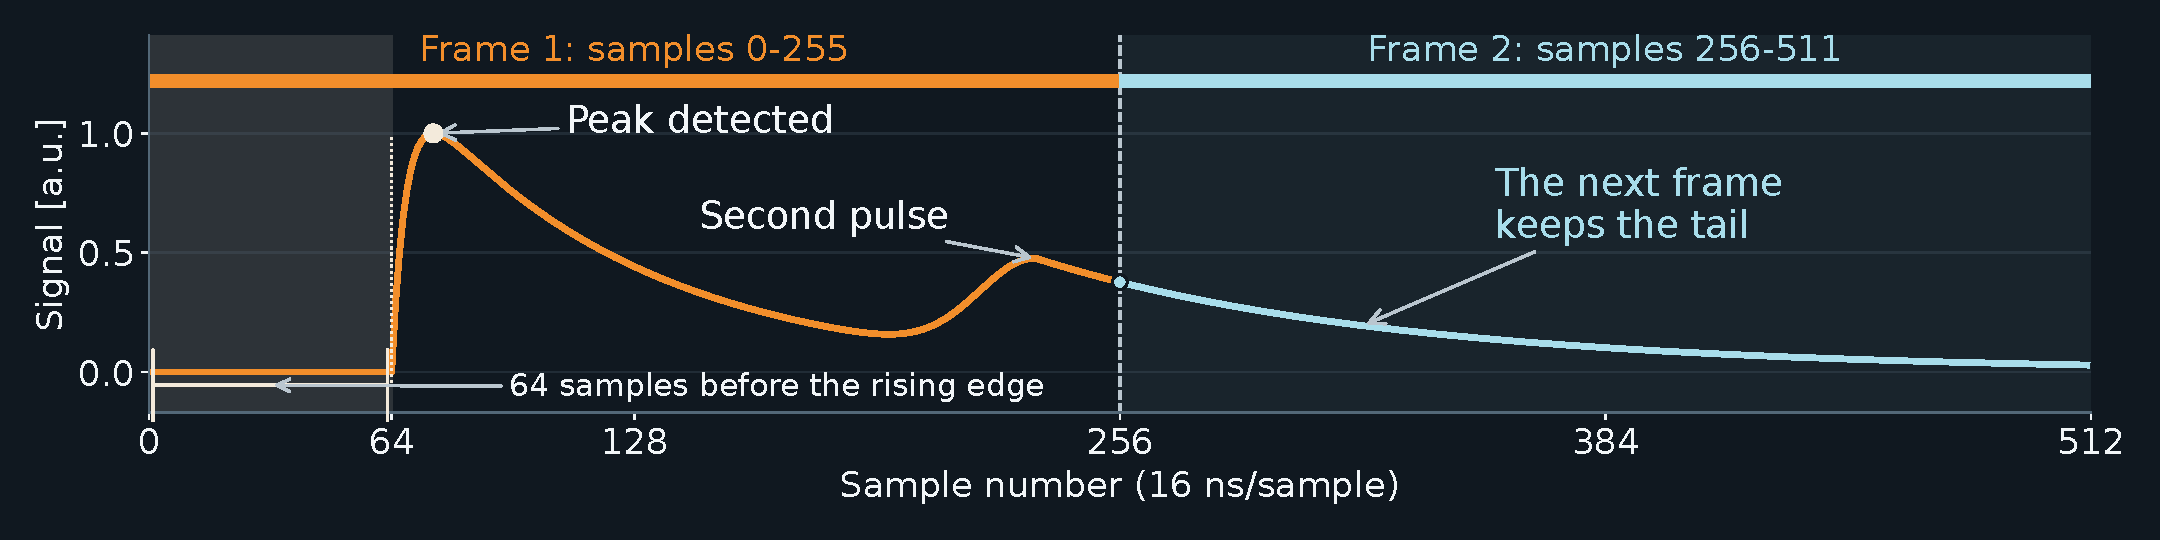
\includegraphics[width=\textwidth,height=0.55\textheight,keepaspectratio]{figures/pulse-windows.pdf}\par
  \bigskip
  {\large Still active? Continue from sample 256.\\No new trigger is needed.\par}
  \medskip
  \DuneDiagramCaption{Illustration adapted from the grouped32 study. Continuation enabled, with buffer space available.\\Consecutive saved samples; queued assembly and readout.}
\end{frame}

% Final -- Pilot comparison; keep the model boundary visible.
\begin{frame}{Two links look promising at the expected activity}
  \centering
  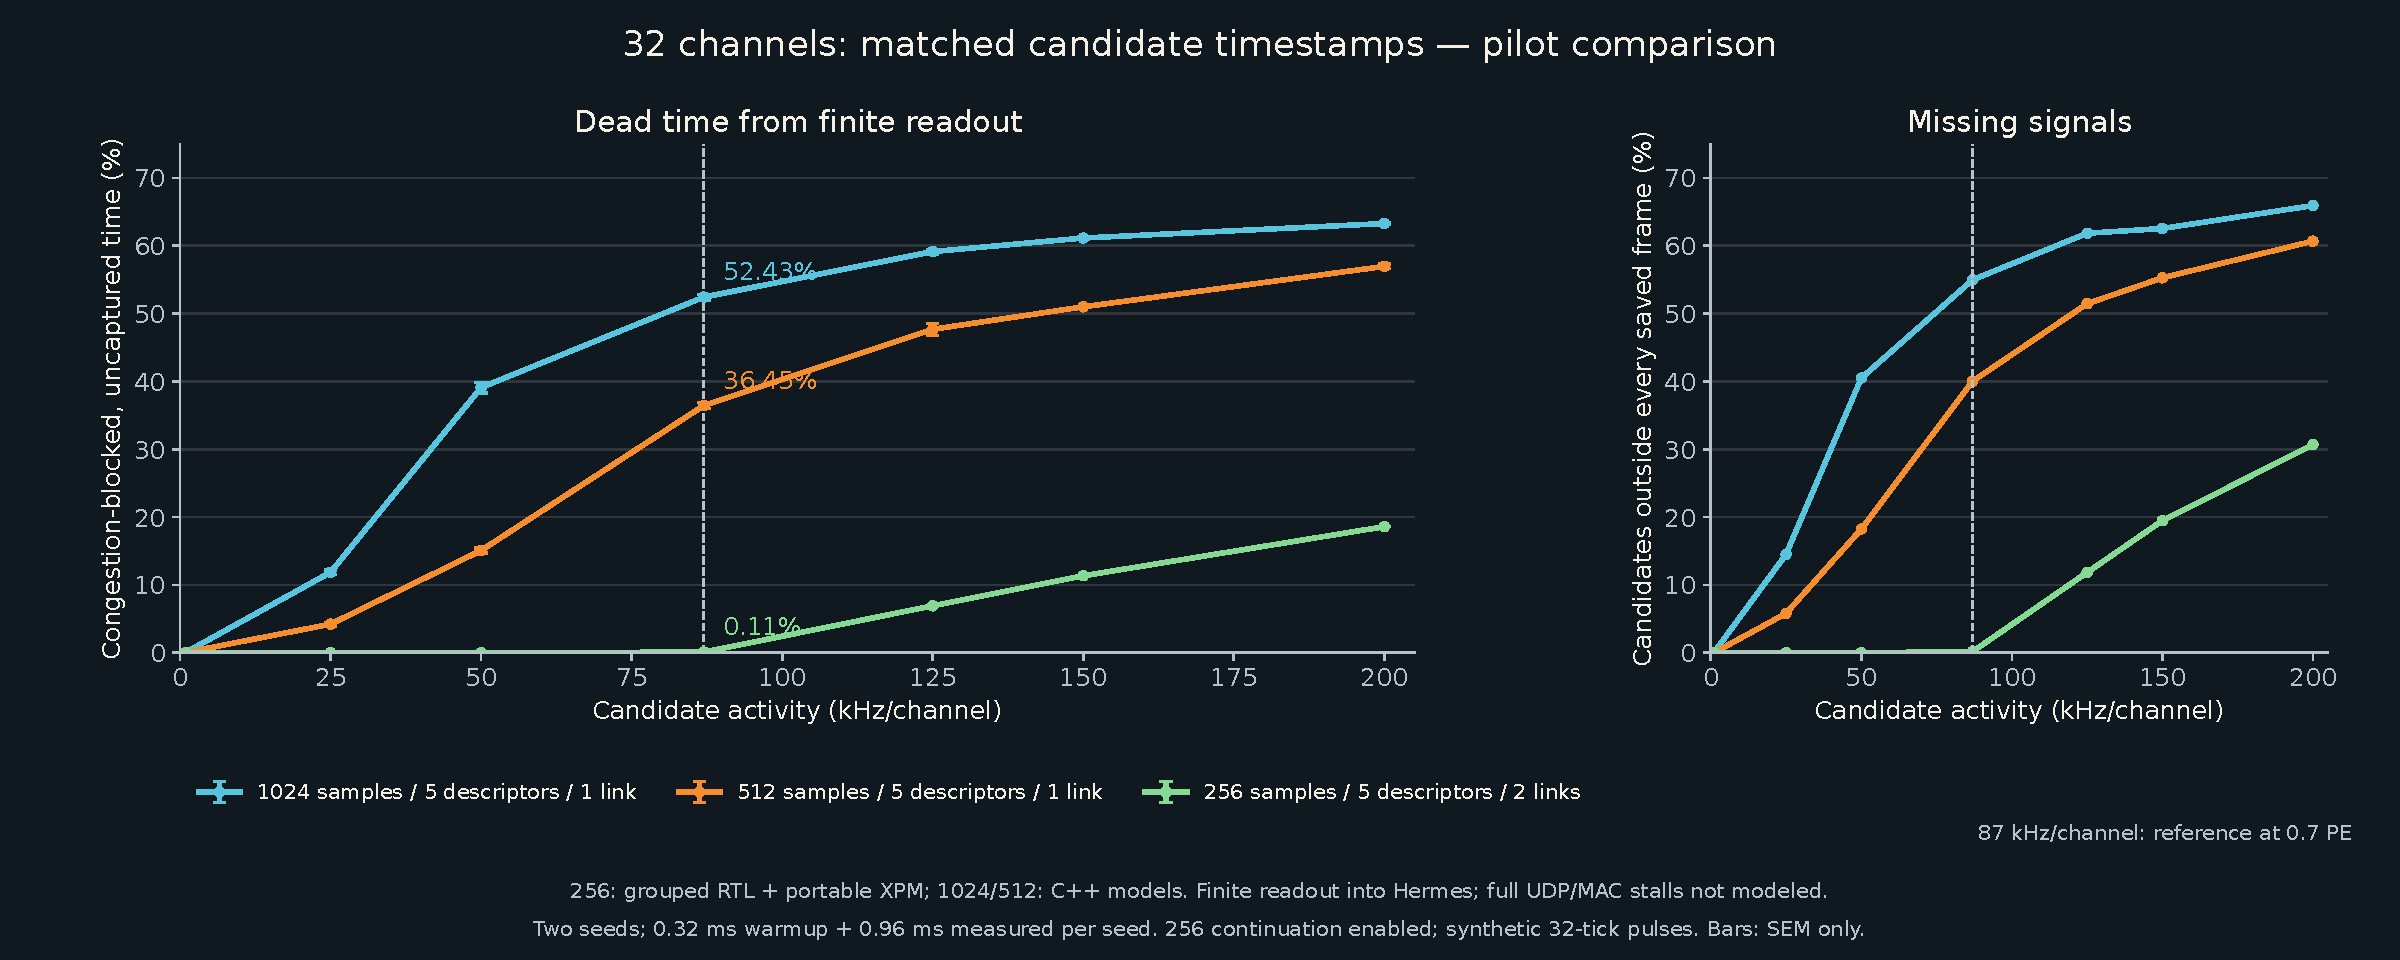
\includegraphics[width=\textwidth,height=0.76\textheight,keepaspectratio]{figures/comparison_256_5_2_pilot.pdf}\par
  \smallskip
  {\small At 87 kHz/channel: 256 / 5 / 2 gives 0.11\% congestion dead time in this pilot.\par}
\end{frame}

% Backup section retained in source, excluded from the PDF.
% \appendix
% \DuneSectionPage{BACKUP}{Study context, packet sizes and model limits}
% 
% % Backup (former slide 7) -- Physics goal, not an efficiency claim.
% \begin{frame}{The smallest pulses are worth keeping}
%   \DuneBigStatement{SINGLE PHOTOELECTRONS: THE SMALLEST LIGHT SIGNALS}
%     {Raising the threshold\\could throw away useful light.}
%     {That light may help us reject backgrounds\\and use more of the detector for physics.}
%   \bigskip
%   {\small\color{DuneTextMuted}A larger usable, or fiducial, volume is the goal. The gain still needs to be measured.}
% \end{frame}
% 
% % Backup (former slide 8) -- The work done, with an explicit evidence boundary.
% \begin{frame}{We tested the problem from C++ to gateware}
%   \centering
%   \begin{tikzpicture}
%     \node[storybox,fill=DunePaper,text width=2.8cm,minimum height=1.9cm] (cpp) at (0,0)
%       {\textbf{C++ models}\\[3pt]Try rates and\\frame formats};
%     \node[storybox,fill=DuneSky,text width=2.8cm,minimum height=1.9cm] (hdl) at (4.4,0)
%       {\textbf{HDL simulation}\\[3pt]Check peaks, buffers\\and stalled output};
%     \node[storybox,fill=DuneCoral,text width=2.8cm,minimum height=1.9cm] (fpga) at (8.8,0)
%       {\textbf{Gateware builds}\\[3pt]Check FPGA space\\and timing};
%     \draw[storyarrow] (cpp) -- (hdl);
%     \draw[storyarrow] (hdl) -- (fpga);
%   \end{tikzpicture}\par\bigskip
%   {\large Rate scans find the limits. HDL checks the logic. Builds check it fits.\par}
%   \medskip
%   \DuneDiagramCaption{Grouped32 RTL replay: 379,656 descriptor words checked. Detector-wide losses below come from the C++ model.}
% \end{frame}
% 
% % Backup (former slide 9) -- Measured VD source traces replayed with output FIFO and lane drain.
% \begin{frame}{One link: the VD activity fills the output FIFO}
%   \small
%   \renewcommand{\arraystretch}{1.45}
%   \begin{tabularx}{\textwidth}{@{}Xrr@{}}
%     \toprule
%     \textbf{Full-VD model result} & \textbf{1024 / 5} & \textbf{512 / 5} \\
%     \midrule
%     Dead time, intrinsic backgrounds & 34.60\% & 21.54\% \\
%     Signals outside every saved frame & 43.36\% & 28.61\% \\
%     New-frame requests rejected & 72.09\% & 55.00\% \\
%     \bottomrule
%   \end{tabularx}
%   \bigskip
%   {\large Shorter frames reduce the modeled loss with one link.\par}
%   \medskip
%   {\small\color{DuneTextMuted}
%     All 1,344 VD channels; 32 channels/board; eight 8.5-ms windows. C++ FIFO/readout model, not RTL validation.\\
%     Threshold $>0.7$ PE. Rates vary across VD; 87 kHz/channel is the cathode reference. Signals here mean threshold candidates.}
% \end{frame}
% 
% % Backup (former slide 12) -- One decision: agree selection before overloading the link.
% \begin{frame}{On one link, we must agree what gets through}
%   \renewcommand{\arraystretch}{1.75}
%   \begin{tabularx}{\textwidth}{@{}p{0.35\textwidth}X@{}}
%     \textcolor{DuneSky}{\textbf{Frame format}} & Shorter frames keep five peak slots and use less bandwidth.\\
%     \textcolor{DuneSky}{\textbf{Readout admission}} & Buffer short bursts; agree which frames pass when the queue fills.\\
%     \textcolor{DuneSky}{\textbf{Trigger logic}} & Use coincident peaks to select useful activity before sending.\\
%   \end{tabularx}
%   \bigskip
%   {\large Preserve weak light; make any selection explicit with DAQ.\par}
%   \medskip
%   {\small\color{DuneTextMuted}Proposals for DAQ agreement. To reduce link traffic, selection must happen before transmission.}
% \end{frame}
% 
% % Backup (former slide 15) -- Close with the agreement and its concrete measurement.
% \begin{frame}{Let's agree how much signal we can afford to lose}
%   \DuneBigStatement{PDS + DAQ}
%     {Choose what to read out,\\how to trigger, and how many links.}
%     {Then replay the same signals through the full chain\\and measure what survives.}
%   \bigskip
%   {\large\color{DuneSky}The test: keep weak pulses, their timing and their charge.\par}
% \end{frame}
% 
% 
% \begin{frame}{Frame formats and packet sizes}
%   \small
%   \renewcommand{\arraystretch}{1.35}
%   \begin{tabularx}{\textwidth}{@{}lrrrr>{\raggedright\arraybackslash}X@{}}
%     \toprule
%     Format & Samples & Sample words & Other words & Total & Contents \\
%     \midrule
%     1024 baseline & 1024 & 224 & 8 & \textbf{232 words / 1,856 B}
%       & Existing header and peak information \\
%     512 study & 512 & 112 & 8 & \textbf{120 words / 960 B}
%       & Same fixed-record structure \\
%     256 / 5 & 256 & 56 & 7 & \textbf{63 words / 504 B}
%       & Two common headers + five descriptors \\
%     \bottomrule
%   \end{tabularx}
%   \bigskip
%   {\large Samples are packed at 14 bits; one output word is 64 bits.\par}
%   \medskip
%     {\small\color{DuneTextMuted}
%     Boundary: DAPHNE frame words presented to Hermes. Hermes, UDP and Ethernet envelopes are not counted. The 256 / 5 packet size is known; its VD loss is not measured.}
% \end{frame}
% 
% \begin{frame}{Inputs to the VD activity estimate}
%   \small
%   \renewcommand{\arraystretch}{1.45}
%   \begin{tabularx}{\textwidth}{@{}p{0.28\textwidth}>{\raggedright\arraybackslash}X@{}}
%     \textcolor{DuneSky}{\textbf{Simulation}} &
%       dunesw v10\_22\_00d01; full VD-v7 geometry. \\
%     \textcolor{DuneSky}{\textbf{Intrinsic sources}} &
%       \(^{39}\)Ar at 0.964 Bq/kg, plus \(^{85}\)Kr, \(^{42}\)Ar and \(^{42}\)K. \\
%     \textcolor{DuneSky}{\textbf{Candidate threshold}} &
%       Strictly above 0.7 photoelectrons; no 10-MeV cut. \\
%     \textcolor{DuneSky}{\textbf{Pulse model}} &
%       Sixteen measured Waffles NP02 cathode-C SPE templates. \\
%     \textcolor{DuneSky}{\textbf{Exposure}} &
%       Eight independent 8.5-ms windows for VD. \\
%   \end{tabularx}
%   \bigskip
%   {\large Result used in the talk: 87,467 candidates/s/channel\\for the VD cathode, before firmware losses.\par}
% \end{frame}
% 
% \begin{frame}{Scope of the gamma estimate}
%   \begin{columns}[T,onlytextwidth]
%     \begin{column}{0.47\textwidth}
%       {\large\color{DuneSky}\textbf{Included in the pilot}\par}
%       \medskip
%       Cavern-wall gammas\\
%       Foam gammas\\
%       Cryostat neutron-gammas\\
%       Cavern neutron-gammas
%     \end{column}
%     \begin{column}{0.47\textwidth}
%       {\large\color{DuneCoral}\textbf{Still open}\par}
%       \medskip
%       Independent repetitions\\
%       Actual cavern neutrons\\
%       Remaining radon components\\
%       Validated electronics-noise rate
%     \end{column}
%   \end{columns}
%   \bigskip
%   {\large One window per source family raises the VD cathode estimate\\
%     from 87,467 to about 92,383 candidates/s/channel.\par}
%   \medskip
%   {\small\color{DuneTextMuted}
%     Candidate timestamps were overlaid before the busy gate; analog waveform pileup was not rebuilt.}
% \end{frame}
% 
% \begin{frame}{How capture dead time must be counted}
%   \small
%   \renewcommand{\arraystretch}{1.42}
%   \begin{tabularx}{\textwidth}{@{}p{0.28\textwidth}>{\raggedright\arraybackslash}X@{}}
%     \textcolor{DuneSky}{\textbf{Saved samples}} &
%       Combine the time intervals covered by all retained frames, including pretrigger and continuation. \\
%     \textcolor{DuneSky}{\textbf{Dead intervals}} &
%       Count only blocked intervals outside that coverage. Live waiting time is excluded. \\
%     \textcolor{DuneSky}{\textbf{Percentage}} &
%       Divide the uncovered blocked time by the full observation time, summed over channels. \\
%     \textcolor{DuneSky}{\textbf{Full-VD result}} &
%       With one link: 34.60\% dead time for 1024 / 5; 21.54\% for 512 / 5, intrinsic activity. \\
%   \end{tabularx}
%   \smallskip
%   {\scriptsize For intrinsic VD input, 3,769,803 / 5,228,561 (1024 / 5) and 2,876,098 / 5,228,561 (512 / 5) new-frame requests were refused. The corresponding candidate timestamps absent from all retained frames were 2,267,339 and 1,496,057. A refused trigger can still lie inside another saved waveform.\par}
%   \smallskip
%   {\small\color{DuneTextMuted}
%     C++ architecture model: FIFO admission and lane drain included; completed frames enter FIFO occupancy as a block. Downstream Hermes stalls and RTL timing are not modeled. Full VD means 1,344 channels on 42 modeled boards.}
% \end{frame}
% 
% \begin{frame}{What buffering and continuation change}
%   \renewcommand{\arraystretch}{1.55}
%   \begin{tabularx}{\textwidth}{@{}p{0.23\textwidth}p{0.34\textwidth}>{\raggedright\arraybackslash}X@{}}
%     \toprule
%     Mechanism & What it protects & Limit \\
%     \midrule
%     \textcolor{DuneSky}{\textbf{Sample ring}} &
%       Recent samples while a frame is assembled &
%       Finite history; old samples are overwritten \\
%     \textcolor{DuneSky}{\textbf{Frame queue}} &
%       Complete frames during a short output stall &
%       Long stalls fill the queue \\
%     \textcolor{DuneSky}{\textbf{Continuation}} &
%       The tail of a pulse beyond the first 512 samples &
%       Every extra frame consumes link bandwidth \\
%     \bottomrule
%   \end{tabularx}
%   \bigskip
%   {\large These features reduce avoidable loss. They do not create output capacity.\par}
% \end{frame}
% 
% \begin{frame}{Four-link mapping and sender budget}
%   \small
%   \renewcommand{\arraystretch}{1.35}
%   \begin{tabularx}{\textwidth}{@{}lccc>{\raggedright\arraybackslash}X@{}}
%     \toprule
%     Link & Channels & Lanes & 512 budget & Constraint \\
%     \midrule
%     0 & 0--7 & 0, 1 & 7.869 Gbit/s & Independent sender \\
%     1 & 8--15 & 2, 3 & 7.869 Gbit/s & Independent sender \\
%     2 & 16--23 & 4, 5 & 7.869 Gbit/s & Independent sender \\
%     3 & 24--31 & 6, 7 & 7.869 Gbit/s & Independent sender \\
%     \bottomrule
%   \end{tabularx}
%   \bigskip
%   {\large Total 512-sender budget: 31.475 Gbit/s across four links.\par}
%   \medskip
%     {\small\color{DuneTextMuted}
%     Traffic cannot move between links. The 256 / 5 production mapping uses eight lanes and four links. Its VD-trace loss is not measured by the C++ legacy model. Values are frame words into Hermes with output ready; network overhead and outages are excluded.}
% \end{frame}
% 
\end{document}
